\documentclass[letterpaper, 12pt]{article}

\usepackage{graphicx}
\usepackage[margin=1.0in]{geometry}

\setlength{\parskip}{0.25cm}

%===================================================
%				Header setup
%===================================================
\newcommand{\myDate}{21 October 2014}
\newcommand{\name}{Rick Sullivan}

%===================================================
%				Boilerplate heading
%===================================================
\title{Aesthetic analysis - Bootstrap framework}
\author{Rick Sullivan}
\date{21 October 2014}

\begin{document}
\begin{center}
\large{Aesthetic analysis - Bootstrap framework}

\normalsize{Rick Sullivan}

\myDate    
\end{center}

\vspace{2 ex}

%==============
%		Body content
%==============

%	intro
Designing web pages is a notoriously arduous process. Web frameworks and website building products that aim to solve the difficulties of web page design have become much more prolific and successful in recent years. I will be analyzing the design of the Bootstrap framework, one of the original web frameworks, which completely changed the way websites are designed and constructed.

%	Functionality and design

The Bootstrap web framework provides a library of user interface elements that users can use to quickly build a simple, but functional website. I will separate my analysis of the design of the framework by first looking at the visual design of the UI elements, and then taking a look at how the framework is designed from a usability standpoint.

\begin{figure}[H]
\centering

\includegraphics{buttons.png}
\caption{The Bootstrap buttons are simple, yet have become ubiquitous on today's Web.}
\end{figure}

\begin{figure}[H]
\centering
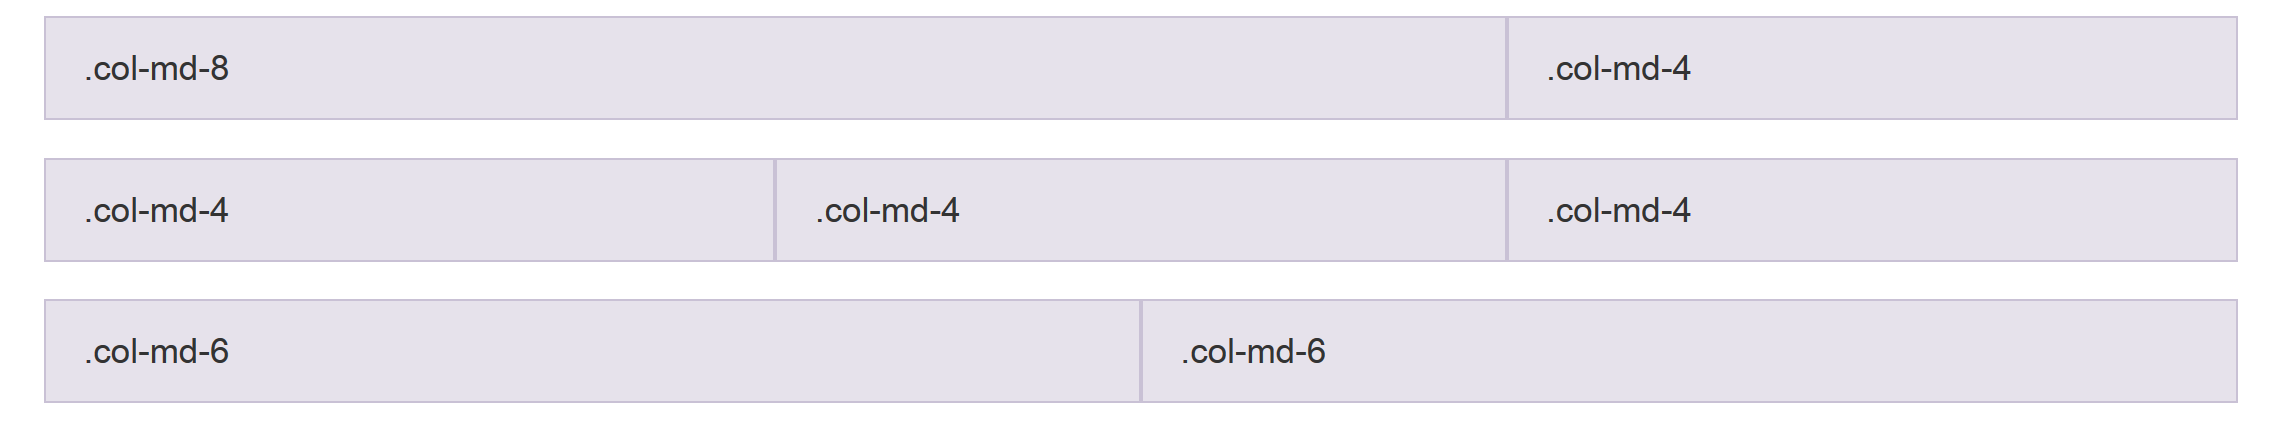
\includegraphics[width=\textwidth]{grid.png}
\caption{Bootstrap provides column and row based formatting. This grid has become the industry standard and is mimicked by many new frameworks.}
\end{figure}

\begin{figure}[H]
\centering
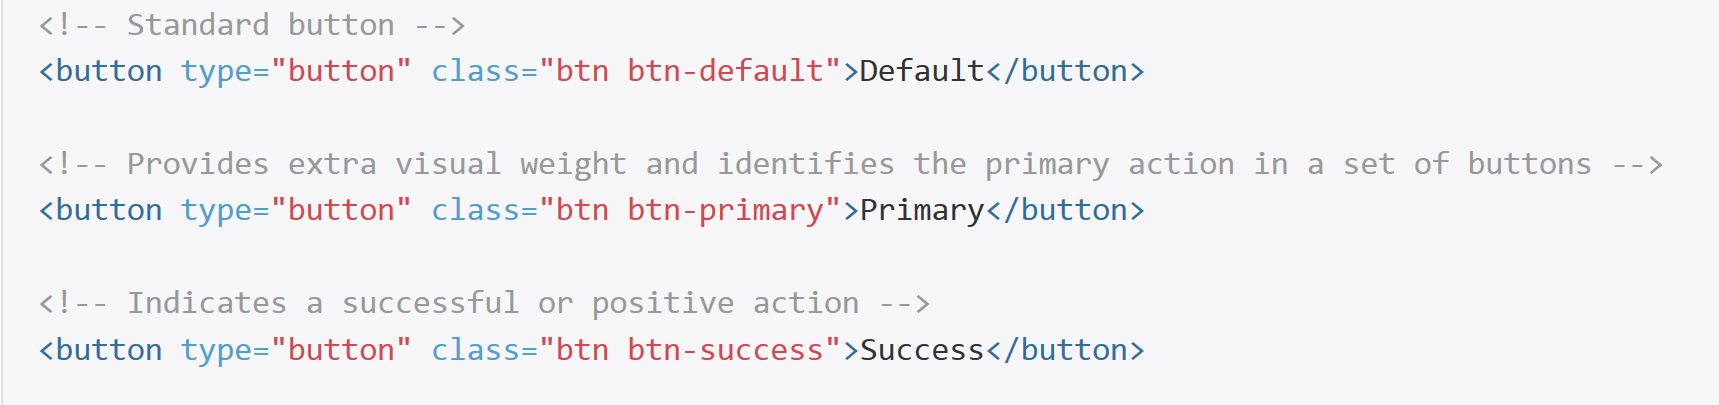
\includegraphics{buttonCode.png}
\caption{Bootstrap is very easy to add to an existing project, with only a minimal amount of code change necessary.}
\end{figure}

%	Standardization and ease of use

%			only a single package 

%	Customizeable and extensible


\end{document}